\documentclass{article}
\usepackage{graphicx}
\usepackage{hyperref}



\begin{document}

\title{Razor Run 2 Analyzer Tutorial}
\author{Javier Duarte, Dustin Anderson}
\maketitle

\tableofcontents

\section{Introduction}
This tutorial is an introduction to the Caltech RazorAnalyzer package for Run
2 CMS data analyses. This code is located on GitHub at
\url{https://github.com/RazorCMS/RazorAnalyzer}. In this tutorial, we
will loop over simulated events and make, display, and compare distributions of event
variables, including the missing transverse momentum (MET), an
important quantity for beyond-the-standard-model (BSM) searches.

\section{Accessing GitHub Code}
To access the code, make an account on \url{https://github.com} (and
email us your username, although that's not necessary to access the
code).

Make sure \textsc{ROOT} is set up properly. Go to a working directory and clone the repository from GitHub.
\begin{verbatim}
git clone https://github.com/RazorCMS/RazorAnalyzer.git
cd RazorAnalyzer
make -j 4
\end{verbatim}
This will compile the code, and may take a while.


\section{Running the Dummy Analysis}
We will edit the analysis code
\texttt{RazorAnalyzer/analyses/DummyAnalysis.cc}. First, we will get
this analysis running, by doing the following. Download the file
located at
\url{https://www.dropbox.com/s/0yrtvzmyz37yjbg/razorNtuple_1.root?dl=1},
which contains simulated top quark-antiquark production plus
associated jets ($t\bar{t}$+jets)
events. Place it in the location \texttt{\textasciitilde/Downloads/razorNtuple\_1.root}.

Now we will make a list of input files for our analysis (consisting
just of this one file). Starting from the same \texttt{RazorAnalyzer}
directory as before,
\begin{verbatim}
echo ~/Downloads/razorNtuple_1.root > lists/test.txt
\end{verbatim}
which creates our desired text list of input files.


As a first task, look through the file
\texttt{RazorAnalyzer/include/RazorEvents.h}. This contains a list of
all the event variables available in the input file. For example,  the variable \texttt{nJets} is the nuber of jets in the
event. The variable \texttt{jetPt} is the transverse momentum (transverse with
respect to the beam line) of a particular jet
in the event. Since there may be many jets in an event, this variable is
actually represented by an array (with one entry for each jet) in the
data file.  Finally, the variable \texttt{metPt} is the missing
transverse momentum (MET) of the event, defined (to first
approximation) as the magnitude of the vectorial sum of the transverse
momenta of all the jets (actually, all particles) in the event.

To run the dummy analysis code the first time (with no changes), we simply do
\begin{verbatim}
./RazorRun lists/test.txt dummy 0
\end{verbatim}
If this command succeded, you should see a printout (one line for each
event) with the value of the MET and the number of jets for each event.


\section{Plotting and Verifying MET}
Now, we would like to edit the code to verify the definition of MET by
making a few histograms: the distribution of the number of
jets, the MET, and the magnitude of the vectorial sum of the transverse
momentum of all the jets. If we've done it correctly, the final two
histograms should be very similar.

First add the following include statements to
\texttt{RazorAnalyzer/analyses/DummyAnalysis.cc} near the top of the
file after the include statement already there.
\begin{verbatim}
#include "TH1D.h"
#include "TFile.h"
#include "TMath.h"
\end{verbatim}

Next, we add the histogram declarations outside of the event for loop after the \texttt{if (fChain
  == 0) return;} statement.
\begin{verbatim}
    //Define new histograms
    TH1D* h_njets = new TH1D("h_njets","njets histogram", 15, 0, 15);
    TH1D* h_met = new TH1D("h_met","MET histogram", 100, 0, 1000);
    TH1D* h_vecjetpt = new TH1D("h_vecjetpt","vecjetpt histogram", 100, 0, 1000);
\end{verbatim}

Now, inside the event for loop, we add the following to fill the
number of jets and MET histograms.
\begin{verbatim}
	//Fill the histograms 
	h_njets->Fill(nJets);
	h_met->Fill(metPt);
\end{verbatim}

To compute the magnitude of the vectorial sum of the transverse momenta of the jets, we
actually need another for loop. Convince yourself that adding the
following code is one correct way to do it. Note how the variables\texttt{vecjetpx}
and \texttt{vecjetpy} are defined in terms of the variables
\texttt{jetPt} and \texttt{jetPhi}. Make sure this makes sense to you
in terms of the coordinate system of CMS.
\begin{verbatim}
	double vecjetpx = 0;
	double vecjetpy = 0;
	for (int iJet=0; iJet<nJets; iJet++){
	  vecjetpx += jetPt[iJet]*TMath::Cos(jetPhi[iJet]);
	  vecjetpy += jetPt[iJet]*TMath::Sin(jetPhi[iJet]);
	}	
	h_vecjetpt->Fill( TMath::Sqrt(vecjetpx*vecjetpx + vecjetpy*vecjetpy) );
\end{verbatim}


Finally, we add the following code after the event for loop is closed, in order to
write out the histograms we've just created.
\begin{verbatim}
    TFile* output = TFile::Open("output.root","recreate");
    output->cd();
    h_njets->Write();
    h_met->Write();
    h_vecjetpt->Write();
    output->Close();
\end{verbatim}

To run this edited code we have to re-compile the package and re-run
the code,
\begin{verbatim}
make
./RazorRun lists/test.txt dummy 0
\end{verbatim}

If you open the output root file that we've just created, 
\begin{verbatim}
root -l output.root
\end{verbatim}
you can plot the histogram by typing \texttt{h\_met->Draw()} at the
\textsc{ROOT} prompt, as seen in Fig.~\ref{fig:met}. Compare this histogram with the one you get by
typing \texttt{h\_vecjetpt->Draw()} instead. Are they similar? If there
are differences, can you think of some reasons for them? Recall the
sample of events we're considering ($t\bar{t}$+jets) and how the top
quark decays (you can look this up on the Particle Data Group webpage).

\begin{figure}
    \centering
    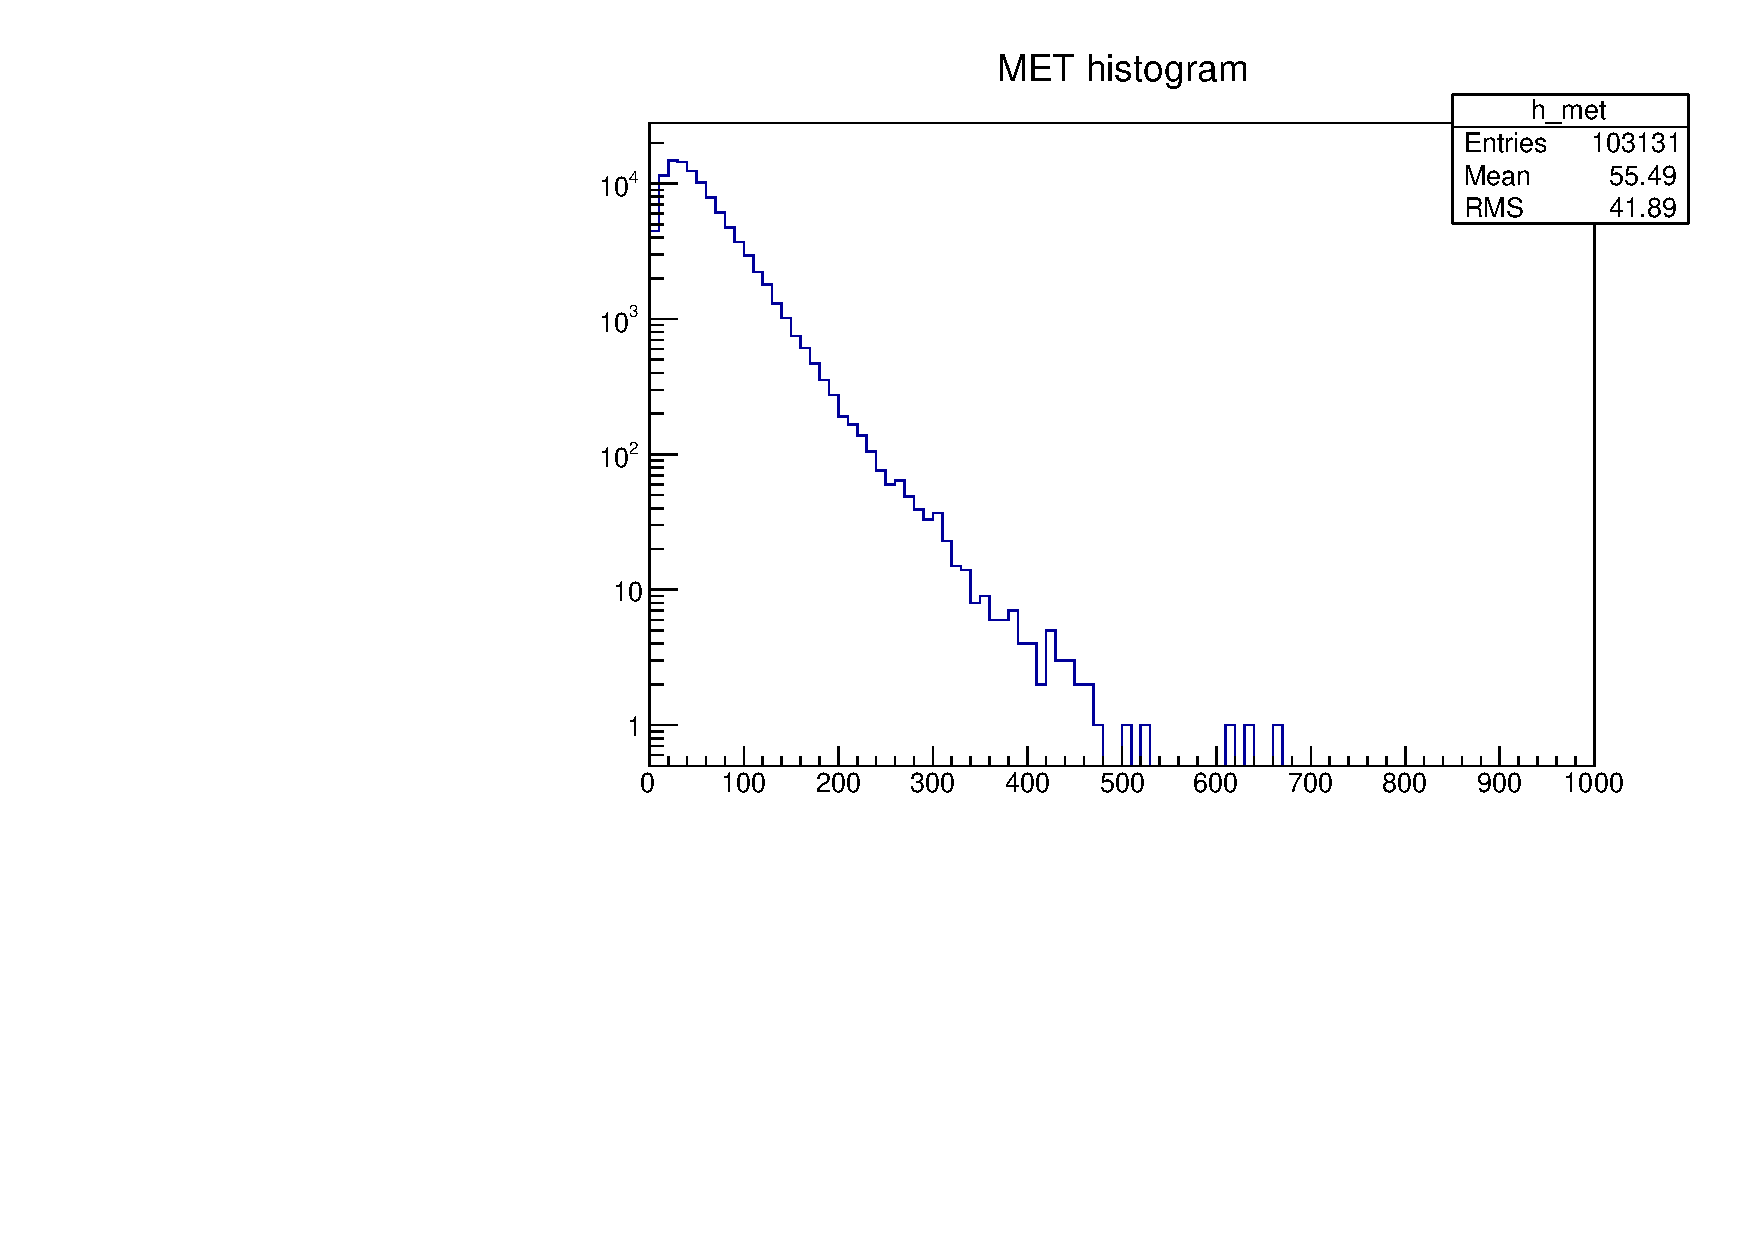
\includegraphics[width=3.0in]{met.pdf}
    \caption{MET distribution in log scale for simulated $t\bar{t}$+jets events}
    \label{fig:met}
\end{figure} 


\end{document}
